\documentclass[a4paper]{article}

\title{Project Implementation
\\COS 301 Buzz Project
\\Group: Testing Phase: Resources
\\Version 1.0}

\author{
\\
\\Carla de Beer 95151835
\\Prenolan Govender 13102380
\\Shaun Meintjes 13310896
\\Collins Mphahlele 12211070
\\Dumisani Msiza 12225887
\\Joseph Murray 12030733
\\Sifiso Shabangu 12081622
\\Joseph Potgieter 12003672
\\Johan van Rooyen 11205131
\\
\\
\textit{https://github.com/Carla-de-Beer/Testing-Resources}
\\
\\ University of Pretoria}

\date{24 April 2015}

% Need to compile using XeLATeX to avoid default font
\usepackage{fontspec}
\setmainfont{Arial}
% Graphics settings for .eps files
\usepackage{graphicx}
\usepackage{epstopdf}
\DeclareGraphicsExtensions{.jpg}
\usepackage{float}
\usepackage{hyperref}

\begin{document}

\maketitle
% No page number to cover page
\pagenumbering{gobble}
\newpage
% start page numbering
\pagenumbering{arabic}

% Generate Table of Contents

\tableofcontents
\newpage

\section{Introduction}

The purpose of this task was to test the functionality provided by the Resources teams for the Buzz Project.
\\
\\
According to the master specification document, version 0.1, released 13 March 2015 (SOLMS \textit{et al}, 2015), the buzzResources module is used to upload and manage resources like media (e.g. images, video) and documents (e.g. PDF documents, Open Document Format documents). These resources are to be either embedded or linked to in posts.
\\
\\
This team took each of the pre and post-conditions of the required use case, considering the work of both Resources A and Resources B, and tested them for compliance with the functional requirements. 
\\
\\The use case for this team is called \textbf{uploadResource}. In terms of the requirements for this use case, and as defined by the master specification document, users should be able to upload resources such as media files or documents. Any uploaded resource should be accessible by other users who should also be able to specify links to that resource. 
\\
\\The functional requirements preconditions for this use case included the need to
\begin{itemize}
\item detect the mime type
\item check that size constraints are met
\item check that the resource type is supported
\end{itemize}
The functional requirements postconditions for this use case included the need to
\begin{itemize}
\item check that the resource persisted
\item check that the URL for the resource was created
\end{itemize}
\textbf{Note to the lecturers: the testing resources group had to import the Resources A code repository into this group's GitHub repository to allow access to the code to all members. This may lead to the appearance of a skew in the git contributions, when this is not the case.}

\section {Functional Testing}

\subsection {Resources A}
\subsubsection {Pre-condition violations}

\paragraph{uploadResources}
\begin{itemize}
\item The mime-type can be detected before the file is uploaded, thus not in violation of condition.
\item The size can be determined before the file is uploaded, also not in violation of pre-condition.
\item The database is queried (albeit erroneously due to logic faults) and checked if the mime-type is supported before the file gets uploaded.
\end{itemize}

\paragraph{getResourcesBySpaceId}
The pre-condition will be that the SpaceID that is sent in as a parameter does exist in the database prior to this execution. There are no violations of this pre-condition.

\paragraph{getResourcesAll}
The pre-condition will be that there exist resources in the database prior to this execution. There are no violations of this pre-condition.

\paragraph{getResourcesRelated}
The pre-condition will be that the appraisal type (RelatedID) that is sent in as a parameter does exist in the database prior to this execution. There are no violations of this pre-condition. 

\paragraph{removeResource}
The pre-conditions which in this case is resource ID being passed as a parameter to removeResource, the ID must exist in the databaase for a resource to be removed.

\paragraph{addResourceType}
The pre-condition will be the MIME type passed would be a valid and existing MIME type and the size limit would be a valid size which would be stated in bytes.

The pre-condition can be violated by passing the MIME type that does not exist and the function will just add the size limit and the MIME type to the Resources contraints in the database.

\paragraph{removeResourceType}
The objectID passed as a parameter must conform to a hexadecimal sequence. If the objectID specified is not hexadecimal, the function returns false.

\paragraph{updateResourceType}
The pre-conditions which in this case is the constraintID passed as a parameter which is the ID of the constraint to be updated must exist in Resources contraints in the database and sizeLimit which is the new size limit of the constraint must be stated in bytes.

\subsubsection {Post-condition violations}

\paragraph{uploadResources}
\begin{itemize}
\item The wrong type of file and file size is added to the database due to improper testing of the mime-type and size.
\item A URL to the resources are not explicitly created, the database needs to be queried each time a resource needs to be found.
\item Persisting resource condition not violated, the resources persist.
\end{itemize}

\paragraph{getResourcesBySpaceId}
The post-condition will be that the resources that exist in a certain space will be returned. This post-condition fails, because the function queries the database and returns all of the resources in the database, which is incorrect. No exceptions are thrown if the Buzz Space does not exist.

\paragraph{getResourcesAll}
The post-condition will be that all of the resources in the database will be returned. This post-condition holds, and all of the resources are returned.

\paragraph{getResourcesRelated}
The post-condition will be that the resources that exist in the database of the specified appraisal type will be returned. This post-condition fails, because the function queries the database and returns all of the resources in the database, which is incorrect.

\paragraph{removeResource}
The post condition will be the removal of the specified resource by ID in the database.

The removeResource does not conform to the post-condition as it cannnot remove the resource that exist in the database with the specified ID.

\paragraph{addResourceType (addConstraint)}
The post-condition is when the size limit and the MIME type would be added to the Resources contraints in the database.

\paragraph{removeResourceType (removeConstraint)}
The objectID which is the ID of the constraint to be removed from Resources contraints in the database will be removed.

\paragraph{updateResourceType (updateConstraint)}
The constraint with the specified constraintID in Resources contraints in the database will be updated by the new size limit.

\subsubsection {Data structure requirements}

\paragraph{uploadResources}
No data structure requirements were given to this function apart from the fact that a timestamp had to be appended to the file name in order to prevent file name clashes. It excels in this area, providing a correct and meaningful timestamp and appending it to the back of the file name.

\paragraph{getResourcesBySpaceId}
No data structure requirements mentioned in the service contract, nor does getResourceBySpaceId utilise any data structures.

\paragraph{getResourcesAll}
No data structure requirements mentioned in the service contract, nor does getResourceAll utilise any data structures..

\paragraph{getResourcesRelated}
No data structure requirements mentioned in the service contract, nor does getResourcesRelated utilise any data structures.

\subsection {Resources B}
None of the functions or use cases for Resources B make use of callbacks.

\textit{ "Nearly everything in node uses callbacks […] Callbacks are functions that are executed asynchronously, or at a later time. Instead of the code reading top to bottom procedurally, async programs may execute different functions at different times based on the order and speed that earlier functions like http requests or file system reads happen."}

\url{github.com/maxogden/art-of-node#callbacks}

The implementation code makes an attempt to allow for the creation of modules for export, but since all the functions, including the main use case, are all object or value-returning functions, it can be said that the code fails, outright, all its services contracts. This is due to the fact that the Resources B code, as it currently stands, cannot be unit tested or integrated into the main code framework for the project. 
The Testing Resources B team undertook an attempt to write unit testing code, working with the existing code structure, rather than amending it other than by introducing a callback to the \texttt{uploadResources} function, in order to be able to test the code for compliance with both functional and non-functional requirements. The code did not run and terminated in an error message stating \texttt{“Error: Cannot find module ‘DataBaseStuff’”}. It seems, therefore that one of the modules is missing from the code structure and, as such, the code could not be tested by means of callbacks.
After some rummaging around in the various GitHub branches, squirrelled away in one of the team members’ branches was a section called “Unit Testing Code”. It became clear that this code is intended to be run via node package manager (npm) and ran unit tests for the following options: 
\begin{itemize}
\item	Download valid resource
\item	Download invalid resource
\item	Add a new Resource Type
\item	Remove a Resource Type
\item	Modify a Resource Type
\item	Retrieve Resource Type Constraints
\item	Detect Mime Type
\end{itemize}
In the absence of being able to test via modules and callbacks, the testing team used this unit test code, as provided by the implementation team, for the testing the Resources B section. Below is a screenshot of the result obtained from the initial running of the provided unit testing code, prior to changing input parameters.

\begin{figure}[H]
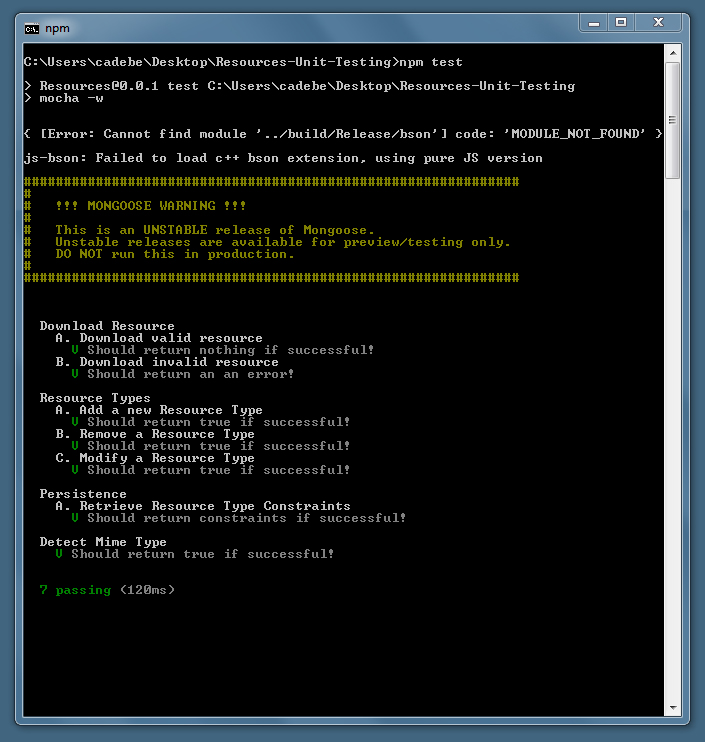
\includegraphics[width=\textwidth]{Images/test-02.jpg}
\caption{Unit testing Resources B: the output provided by running the unit test code, as provided by the implementation team \label{overflow}}
\end{figure}

\subsubsection {Pre-condition violations}

\paragraph{uploadResources} The uploadResources use case function makes an attempt to fulfil the mimetype detection precondition, as well as the \texttt{getResourceTypeConstraints} and throws an exception in the case where
\begin{itemize}
\item the file size constraints have not been met
\item the resource type is not supported
\item the mimetype could not be detected
\end{itemize}
The raising of these exceptions is commensurate with the services contract requirements, as specified in Figure 28 in the master specification document (SOLMS et al, 2015).
There is no actual unit testing code written for the \texttt{uploadResources} use case. Considering that the other functions pertaining to the uploading of resources do not work, it is expected that this function will fail.
In terms of the actual code, the mimetype size is tested by means of the line:

\texttt{	file.size <= (constraints.maximumSize * 1000)}

There is no explanation as to why this particular value has been chosen as the file size constraints. Something similar to the notion of a constant value, declared at the head to the file, might have been more appropriate and explanatory in this case.
In summary, there is an attempt to fulfil the use case pre-conditions by means of inclusion of exceptions for the cases where the preconditions may fail, however, the code fails in cases where erroneous input is added. In such cases the code would have benefited from the application of additional exception throwing to cover these scenarios.

\paragraph{downloadResource} 

This use case calls the line 

\texttt{var results = resources.downloadResource("mountain.jpg");}

and when this line is changed to read

\texttt{var results = resources.downloadResource("mountain");}

the code still executes successfully. It appears that the unit testing for this function is not working correctly, and as such, the use case cannot be tested with the code provided. 

\paragraph{modifyResourceType}
The required pre-conditions for this use case include the need for testing the validity of the mimetype that is sent through, as well as a parameter to limit the size limit the size of the mimetype change, presumably to avoid potential malpractice. The unit testing code as provided by the implementation team was not considered to be reliable in the testing of this use case, and since the modifyResourceType function appears to be a Boolean returning function, rather than actually modifying the specified item in the database, it can be concluded that this use case is violating its required pre-conditions.

\paragraph{addResourceType}
The pre-condition of addResourceType is assumed to be valid data. Tests for empty strings and resource types that do not belong to the MIME types were passed, without exceptions being thrown.

\paragraph{removeResourceType}
The pre-condition of removeResourceType is assumed to be valid data. Tests for empty strings and resource types that do not belong to the MIME types were passed, without exceptions being thrown. There were also no exceptions thrown for types that have not been added.

\paragraph{removeResource}
The pre-condition of removeResource is assumed to refer to the identification number of a resource in the database which should exist prior to this execution. There are no violations of this pre-condition due to error checks being performed to verify whether or not the entry exists.

\paragraph{removeResourceTypeConstraint}
The pre-condition of removeResourceTypeConstraint is assumed to be valid data. Tests for empty strings were passed without exceptions being thrown. There were also no exceptions thrown for type constraints that have not been added.

\paragraph{detectMimeType} 
There appears to be problems with the mimetype detection functionality. It is hard to see how this function, as it currently stands, will return a value other than true. Running the provided test code for the “Detect Mime Type” seems to confirm this. Each time the code was run, the code executes without fail when tested against various mimetypes. Representatives from the various mimtype groups were used, with emphasis on the ones that are expected to be most frequently used, including:
\begin{itemize}
\item image/jpeg
\item image/png
\item image/gif
\item image/targa
\item image/svg+xml
\item image/example
\item audio/mp3
\item message/http
\item multipart/alternative
\item multipart/encrypted
\item text/cmd
\item text/csv
\end{itemize}
However, when the line \texttt{var results = mime.detectMimeType("./r/mountain.jpeg");} 

was amended to \texttt{var results = mime.detectMimeType("./r/rubbish");}

the code also happily returned a true value. It seems that neither the the unit testing code for this use case, not the actual use case code, works correctly in that the mimetypes are not correctly detected.

\subsubsection {Post-condition violations}

\paragraph{uploadResources}
There is a folder with images and music files, but the code seems to make the presumption that there is a server in place that can handle the uploads. Since the \texttt{uploadResources} use case was not included in the unit testing, since the unit testing code has proved itself to be defective, and since many of the functionalities, such as mimetype detection, which \texttt{uploadResources} depends on, do not work themselves, it is concluded that the uploading of resources has not persisted to the database. No URLs seems to be created for the uploaded files. 

\paragraph{modifyResourceType}
It is not clear whether the items uploaded to the database are actually persisting. There is a folder with images and music files, but the code seems to make the presumption that there is a server in place that can handle the uploads.

\paragraph{removeResource}
The post-condition of removeResource would be the removal of an entry. Due to a lack of unit testing functionality, the post-condition fails as there is no visible indication of removeResource working.

\paragraph{downloadResource}
Since resources could not be uploaded to the database, resources could consequently not be downloaded.

\paragraph{detectMimeType}
The mimetypes were not correctly identified.

\subsubsection {Data structure requirements}

\paragraph{uploadResources}
The \texttt{uploadResource} use case calls a filepath to an object to be uploaded, rather than an object or data structure itself. No data structures have been specified as required in the master specification document, and none were required.

\paragraph{addResourceType}
No data structure requirements mentioned in the service contract. However, \texttt{addResourceType} requires a string value as the only input. Said string must be a MIME type.

\paragraph{removeResourceType}
No data structure requirements mentioned in the service contract. However, \texttt{removeResourceType} requires a string value as the only input. Said string must be a MIME type.

\paragraph{modifyResourceType}
There are no data structure requirements for this use case.

\paragraph{removeResource}
No data structure requirements mentioned in the service contract, nor does \texttt{removeResource} utilise any data structures.

\paragraph{downloadResource}
The \texttt{downloadResource} use case calls a filepath to an object to be uploaded, rather than an object or data structure itself. No data structures were required for this use case.

\paragraph{detectMimeType}

The \texttt{detectMimeType} use case calls a filepath to an object to be uploaded, rather than an object or data structure itself. No data structures were required for this use case.

\section {Non-functional testing / assessment}
\subsection {Resources A}
The use case was tested against the following list of architectural requirements:
\subsubsection {Usability}

\paragraph{uploadResources}
Usage of this function is fairly easy and obvious. The selected files from the file selector only need to be sent through to the function and it handles all the rest of the heavy lifting. It can handle multiple files at once and tests each file individually.

\paragraph{getResourcesBySpaceId}
This function is easy and simple to use. The function is called with the Space ID, and a list of the resources for that space is returned.

\paragraph{getResourcesAll}
This function is simple and easy to use. The function is called and all resources within the database is returned.

\paragraph{getResourcesRelated}
This function is simple and easy to use. The function is called and an appraisal type is sent as parameter. All resources of that appraisal type is returned.

\subsubsection {Performance}

\paragraph{uploadResources}
The performance of this function would rely on network speed and stable connection to the database, since it does not require much computational time or pc resource allocation.

\paragraph{getResourcesBySpaceId}
This function does not suffer from performance issues. The performance of this function depends on the connection and communication speed of the database.

\paragraph{getResourcesAll}
This function does not suffer from performance issues. The performance of this function depends on the connection and communication speed of the database.

\paragraph{addingConstraint,removeConstraint and updateConstraint}
Connection to the database takes longer adding Constraint response time is unrealistic for the system as it takes longer.

\paragraph{getResourcesRelated}
This function does not suffer from performance issues. The performance of this function depends on the connection and communication speed of the database.

\subsubsection {Scalability}

\paragraph{uploadResources}
This function allows multiple files to be uploaded together, with no specified limit of files. The size of each file is limited by the relevant mime-type entry in the database, thus, theoretically, any file size should be able to be uploaded, if the database permits it. Furthermore, multiple users can use the function concurrently, because of the way the server can be set up.

\paragraph{getResourcesBySpaceId}
This function does not place any restriction on the possible size of the database, as a list of all resources within a certain space is returned.

\paragraph{getResourcesAll}
This function does not place any restriction on the possible size of the database, as a list of all resources in the database is returned.

\paragraph{getResourcesRelated}
This function does not place any restriction on the possible size of the database, as a list of resources of a certain type is returned.

\subsubsection {Testability}

\paragraph{uploadResources}
The testability of this function is not hard at all, since it allows only a certain number of things to happen. If a file is not allowed, it shouldn't be uploaded, if it is, it should. If the file size is too large, likewise. It is quite easy to send a query to the database to see if the correct information was stored by the function, thereby further enhancing the testability thereof.

\paragraph{getResourcesBySpaceId}
This function is easy to test, as it can be tested from the interfaces that was created.

\paragraph{getResourcesAll}
This function is easy to test, as it can be tested from the interfaces that was created.

\paragraph{getResourcesRelated}
This function is easy to test, as it can be tested from the interfaces that was created.

\paragraph{addingConstraint,removeConstraint and updateConstraint}
No unit test created for testing of each functions implemented and provided testing is in the app.js file which caters the interface side of the function,however adding Constraint and other functions result in too long to response exception being thrown by the browser as connection with the database is not well established and fails.

\subsubsection {Security}

\paragraph{uploadResources}
This function does not handle any type of security (except not allowing harmful mime-types). The connection to the database, for instance, is created somewhere else and the database object is only used by this function.

\paragraph{getResourcesBySpaceId}
This function is secure, as it only retrieves information from the database, about the resources for a certain space.

\paragraph{getResourcesAll}
This function is secure, as it only retrieves information from the database, about all of the resources in the database.

\paragraph{getResourcesRelated}
This function is secure, as it only retrieves information from the database, about all of the resources of a certain appraisal type.

\paragraph{addingConstraint}
Interface is not secured in the client side adding Constraint section does not validate user input and adds the given input to the database without any validation ,the only validation is on the server side where it checks if the input is not already in the database.

\subsubsection {Reliability}

\paragraph{uploadResources}
In the cases tested, the function is not reliable as it should be. It allows multiple files to be uploaded, as it should, however - it allows ALL files of any size to be uploaded due to a logic error in the code. The size is tested the wrong way around (a test is done to see if the max size is smaller than the file size, which is wrong). Not only that, a function is used to count the amount of records found, but the object containing all the records found cannot be "counted" in the way the coder wanted to. In order to make sure that the code was indeed faulty, new code was written to test the file to be uploaded and it was found that the original coder had indeed made a mistake.

\paragraph{getResourcesBySpaceId}
This function is very unreliable, because it does not conform to the post-condition. It returns a list of all of the resources, instead of only returning a list of resources within a certain space.

\paragraph{getResourcesAll}
This function is reliable as it conforms to the post-condition. The function returns a list of all of the resources within the database.

\paragraph{getResourcesRelated}
This function is very unreliable, because it does not conform to the post-condition. It returns a list of all of the resources, instead of only returning a list of resources of a certain appraisal type.

\paragraph{addingConstraint,removeConstraint and updateConstraint}
Lack of input validation results in garbage data entered in the database,which result in unreliable results and connection to database takes too long or results in browser throwing an exception for taking too long to respond,thus module is not reliable to complete a task base on this factors.


\subsubsection {Reusability}

\paragraph{uploadResources}
This function can easily be reused, since it keeps no remnants of previous data that can possibly corrupt new data. Each use of the function is thus a clean slate, so to speak. It is also exported as part of the package.

\paragraph{getResourcesBySpaceId}
This function is reusable, as it retrieves information from the database, about the resources for a certain space. This function can be called and reused throughout the system.

\paragraph{getResourcesAll}
This function is reusable, as it only retrieves information from the database, about all of the resources in the database. This function can be called and reused throughout the system.

\paragraph{getResourcesRelated}
This function is reusable, as it only retrieves information from the database, about all of the resources of a certain appraisal type. This function can be called and reused throughout the system.

\subsubsection {Pluggability}

\paragraph{uploadResources}
This function is pluggable to the extent that mongoose is used as an interface to connect to the database. When that requirement is complied with, the function will be portable (it will accept file data and write it to the connected database). Electrolyte is also used to make the function more pluggable.

\paragraph{getResourcesBySpaceId}
This function is pluggable, as it retrieves information from the database, about the resources for a certain space. This function can be called and reused within any system if called on a database that has the same structure as the current database.

\paragraph{getResourcesAll}
This function is reusable, as it only retrieves information from the database, about all of the resources in the database. This function can be called and reused within any system if called on a database that has the same structure as the current database.

\paragraph{getResourcesRelated}
This function is reusable, as it only retrieves information from the database, about all of the resources of a certain appraisal type. This function can be called and reused within any system if called on a database that has the same structure as the current database.


\subsection {Resources B}
The use case was tested against the following list of architectural requirements:
\subsubsection {Usability}

\paragraph{uploadResources}
There is no indication of the provision of HTML elements as part of the implementation team’s work, so it can’t be stated with certain how this use case is intended to be implemented in terms of an interface. However, the function is designed to be fairly simple to use: the user calls this function, supplying input values that provide the file path to the object to be uploaded, and a short description thereof.

\paragraph{downloadResource}
 The function is intended to be fairly simple and easy to use: only a file name is required.

\paragraph{modifyResourceType}
Since the function does not work as required, any associated performance measurement, in this case, is irrelevant. 

\paragraph{removeResource}
removeResource demonstrates usability by being simple and easy to use. The function only needs be called along with the ID of the resource to be removed which is intuitive.

\paragraph{addResourceType}
addResourceType demonstrates usability by being simple and easy to use. The function only needs be called along with the string name of the resource to be added which is intuitive.

\paragraph{removeResourceType}
removeResourceType demonstrates usability by being simple and easy to use. The function only needs be called along with the string name of the resource to be removed which is intuitive.

\paragraph{retrieveResourceTypeConstraint}
retrieveResourceTypeConstraint demonstrates usability by being simple and easy to use. The function only needs be called along with the string name of the resource of which the constraint should be retrieved which is intuitive.

\paragraph{detectMimeType}
Again, without an indication of interface design for this use case, it can’t be stated with certainty what the usability implications would be. However, from the parameter requirement for this function, i.e. the input of a file path, the intention is for a fairly straightforward and simple use.

\subsubsection {Performance}

\paragraph{uploadResources}
It is hard to measure the performance of this code accurately. Since the general impression is that the code is not working correctly, the execution time given at the bottom of the screen for each of the test runs is somewhat meaningless. Even if it were useful, there is no benchmark available from Resources A, for example, against which to test the performance of this use case.

\paragraph{downloadResource}
It is hard to measure the performance of this code accurately. Since the general impression is that the code is not working correctly, the execution time given at the bottom of the screen for each of the test runs is somewhat meaningless. However, the function is merely downloading a resource from a server, and performance for the majority of files, assuming that they are fairly small, should be fairly efficient for this use case.

\paragraph{removeResource}
removeResource does not suffer from any performance issues in and of itself, however should the database maintain a sizeable stature, removeResource will be seen to suffer in performance. This is to be expected.
performance

\paragraph{addResourceType}
addResourceType does not suffer from any performance issues in and of itself, however should the database maintain a sizeable stature, addResourceType will be seen to suffer in performance. This is to be expected.
performance

\paragraph{removeResourceType}
removeResourceType does not suffer from any performance issues in and of itself, however should the database maintain a sizeable stature, removeResourceType will be seen to suffer in performance. This is to be expected.
performance

\paragraph{retrieveResourceTypeConstraint}
retrieveResourceTypeConstraint does not suffer from any performance issues in and of itself, however should the database maintain a sizeable stature, retrieveResourceTypeConstraint will be seen to suffer in performance. This is to be expected.

\paragraph{detectMimeType}
The function is a Boolean returning value, and such, had it been correctly implemented, should have been reasonably efficient. 

\subsubsection {Scalability}

\paragraph{uploadResources}
A limit has been imposed on the size of files that can be uploaded, therefore scalability in terms of upload size is restricted. The function is designed to upload only a single file at any one time.

\paragraph{downloadResource}
There should not be any issues with regard to scalability of this use case - the only burden might be on the server.

\paragraph{modifyResourceType}
A size limit is imposed on the degree of modification that can be made to the uploaded resource, as such there is a limitation on the scalability of modifications that can be made.

\paragraph{removeResource}
removeResource offers no solutions to accomodate an increase or decrease in size of the database.

\paragraph{addResourceType}
addResourceType offers no solutions to addResourceType an increase or decrease in size of the database.

\paragraph{removeResourceType}
removeResourceType offers no solutions to removeResourceType an increase or decrease in size of the database.

\paragraph{retrieveResourceTypeConstraint}
retrieveResourceTypeConstraint offers no solutions to retrieveResourceTypeConstraint an increase or decrease in size of the database.

\paragraph{detectMimeType}
Scaling the system up, or down, should not have any implication on this function. 

\subsubsection {Testability}

\paragraph{uploadResources}
Some unit testing has been undertaken by the implementation team; however, as became clear, this code does not work as expected. On a positive note, the use of modularisation does help in separating out functionalities and being able to focus on the individual functions. 

\paragraph{downloadResource}
Some unit testing has been undertaken by the implementation team; however, as became clear, this code does not work as expected. On a positive note, the use of modularisation does help in separating out functionalities and being able to focus on the individual functions. 

\paragraph{modifyResourceType}
The function has been modularised and this should , in principle, facilitate its testability.

\paragraph{removeResource}
removeResource has a complete lack of testability due to it not conforming to proper unit testing standards (making use of callbacks, depending on a live database etc.).

\paragraph{addResourceType}
addResourceType seems to be testable.

\paragraph{removeResourceType}
removeResourceType seems to be testable.

\paragraph{retrieveResourceTypeConstraint}
retrieveResourceTypeConstraint seems to be testable.

\paragraph{detectMimeType}
Some unit testing has been undertaken by the implementation team; however, as became clear, this code does not work as expected: the function returns true regardless of the mimetype input provided. 

\subsubsection {Security}

\paragraph{uploadResources}
There does not seem to be to be any limit imposed on the length of the description to be provided as part of the function parameters. There is the risk that someone could attempt to upload a significant amount of information, potentially malware, onto the server via this input value, potentially causing issues. 

\paragraph{downloadResource}
There should not be any security issues involved in downloading resources from the server.

\paragraph{modifyResourceType}
This function may pose a security risk. It does not check the mimetype to see if it may be harmful. The function also doesn’t place constraints on the new size limit, which could lead to a significant portion of the database’s memory being allocated to the resources.

\paragraph{removeResource}
The only security concern would be an incorrect ID being used in order to remove a different resource than required, potentially putting the system at risk.

\paragraph{addResourceType}
addResourceType has no input validations and is therefore a great security risk.

\paragraph{removeResourceType}
removeResourceType has no input validations and is therefore a great security risk.

\paragraph{retrieveResourceTypeConstraint}
retrieveResourceTypeConstraint has no input validations and is therefore a great security risk.

\paragraph{detectMimeType}
This use case simply checks a file type for validity and, as such, does not pose and security concerns.

\subsubsection {Reliability}

\paragraph{uploadResources}
The use case does not work as expected and can therefore not be described as being 

\paragraph{downloadResource}
The use case does not work as expected and can therefore not be described as being 
reliable. 

\paragraph{modifyResourceType}
The use case does not work as expected and cannot be described as reliable.

\paragraph{removeResource}
According to the failure of the post-condition, removeResource gives a poor indication with regards to reliability.

\paragraph{addResourceType}
According to the failure of the post-condition, addResourceType gives a poor indication with regards to reliability.

\paragraph{removeResourceType}
According to the failure of the post-condition, removeResourceType gives a poor indication with regards to reliability.

\paragraph{retrieveResourceTypeConstraint}
According to the failure of the post-condition, retrieveResourceTypeConstraint gives a poor indication with regards to reliability.

\paragraph{detectMimeType}
This function cannot be considered to be reliable: it returns true regardless of the mimetype input provided. 

\subsubsection {Reusability}

\paragraph{uploadResources}
If the use case does not work, it can be argued that there is no scope for reusability.

\paragraph{downloadResource}
If the use case does not work, it can be argued that there is no scope for reusability.

\paragraph{modifyResourceType}
The use case does not work as expected and cannot be described as reusable.

\paragraph{removeResource}
removeResource is not very reusable due to the dependence on a single database. Using this function throughout this system would not be possible/practical.

\paragraph{addResourceType}
addResourceType is not very reusable due to the dependence on a single database. Using this function throughout this system would not be possible/practical.

\paragraph{removeResourceType}
removeResourceType is not very reusable due to the dependence on a single database. Using this function throughout this system would not be possible/practical.

\paragraph{retrieveResourceTypeConstraint}
retrieveResourceTypeConstraint is not very reusable due to the dependence on a single database. Using this function throughout this system would not be possible/practical.

\paragraph{detectMimeType}
If the use case does not work, it can be argued that there is no scope for reusability.

\subsubsection {Pluggability}

\paragraph{uploadResources}
Due to the absence of use of callbacks in the code, as it currently stands, the code cannot be integrated into the existing implementation structure, and is therefore not pluggable.

\paragraph{downloadResource}
Due to the absence of use of callbacks in the code, as it currently stands, the code cannot be integrated into the existing implementation structure, and is therefore not pluggable.

\paragraph{modifyResourceType}
Due to the absence of callbacks in this code, as it currently stands, the code cannot be integrated into the existing implementation structure and is therefore, cannot be considered to be pluggable.

\paragraph{removeResource}
In the same vein as reusability, removeResource cannot be integrated into other systems due to a lack of robustness and versatility.

\paragraph{addResourceType}
In the same vein as reusability, addResourceType cannot be integrated into other systems due to a lack of robustness and versatility.

\paragraph{removeResourceType}
In the same vein as reusability, removeResourceType cannot be integrated into other systems due to a lack of robustness and versatility.

\paragraph{retrieveResourceTypeConstraint}
In the same vein as reusability, retrieveResourceTypeConstraint cannot be integrated into other systems due to a lack of robustness and versatility.

\paragraph{detectMimeType}
Due to the absence of use of callbacks in the code, as it currently stands, the code cannot be integrated into the existing implementation structure, and is therefore not pluggable.


\section {Critical Evaluation and Recommendations}
\subsection {Resources A}
\subsubsection {Master specification compliance}
The following of the master specification for the implementation was followed correctly to some extent in the resource implementation ,most functions were implemented and worked to some extent,functionality was prioritised over following software principles like having a unit test for each function created and being specific in documentation of functions parameter types .

\subsection {Resources B}
\subsubsection {Code and code structure legibility}
The code has some degree of JSDoc comments, but could have benefited from a more comprehensive commenting system so as to allow newcomers to the code to better understand the program logic. The use of an explanatory README file would also have been welcomed by the testing team and others new to the work to help understand the logic behind the system implemented. Thus, from a code legibility point of view, there are some improvements that can be made to make the existing code more user-friendly. On a positive note, the code does make use of modularisation in the sense the additional functionalities are separated out from the main use case, making it easier to understand, and perhaps also easier to test the code.
In terms of the files themselves, the file structure could have benefited from a better organisational structure. There are files with duplicate naming, for example, residing in different folders, making it unclear how these fit into the existing code structure (it was assume that the code folders in the master branch were the most current).  In addition, the unit testing code was hidden away in a branch and, as such, was not that straightforward to find.

\subsubsection {Use cases}
It seems as though the team added additional use cases to the project, such as removeResourceType, modifyResourceType and removeResourceType, in addition to the required use case uploadResource, and its associated pre and post-conditions. This is a laudable, however, there are issues in the main use case that had not been resolved, and there are also issues with the use cases introduced. In hindsight it might have been more expedient for the implementation team to have focused on correctly implementing the main required use case, and additional functionalities later on if there were time.



\section {References}
SOLMS, F., PIETERSE V., OMELEZE S., RAMASILA, L. 2015. \textit{Buzz Discussion Board Requirements and Design Specifications (version 0.1)}. Department of Computer Science, University of Pretoria.


\end{document}
